\section{Integración elemental de ecuaciones no lineales}

\subsection{Introducción y pérdida de linealidad}

Hasta este punto, nuestro estudio se ha centrado exclusivamente en el ámbito de las ecuaciones y sistemas diferenciales lineales. La estructura lineal nos dotó de propiedades algebraicas muy buenas, siendo entre las más  destacadas el \textit{Principio de Superposición}, el cual nos permitía construir soluciones generales a partir de combinaciones lineales de un conjunto fundamental de soluciones particulares. 

Sin embargo, cuando abandonamos el régimen lineal, esta cómoda estructura algebraica colapsa. Para ilustrar este fenómeno, consideremos la siguiente y ecuación diferencial ordinaria no lineal de primer orden:
\[
    u' = u^2
\]
Esta ecuación no es lineal y, en consecuencia, no cumple el principio de superposición. Podemos demostrarlo rápidamente por reducción al absurdo. Si una función $u(t)$ fuera solución de esta ecuación ($u' = u^2$), y asumiéramos que el principio de superposición sigue vigente, cualquier múltiplo escalar $\lambda u(t)$ también debería ser solución. Sustituyendo en la ecuación diferencial tendríamos:
\[
    (\lambda u)' = (\lambda u)^2 \implies \lambda u' = \lambda^2 u^2
\]
Como sabemos que $u' = u^2$, podemos sustituirlo en el lado izquierdo:
\[
    \lambda (u^2) = \lambda^2 u^2 \implies (\lambda - \lambda^2)u^2 = 0
\]
Para que esta igualdad se cumpla para cualquier solución no trivial ($u \neq 0$), forzosamente tendríamos que $\lambda = \lambda^2$, lo cual solo es cierto si $\lambda = 0$ o $\lambda = 1$. Es decir, el espacio de soluciones ya no es cerrado bajo el producto por escalares. 

De forma análoga, la suma de soluciones falla. Si tomamos dos soluciones $u_1, u_2$ y evaluamos si su suma $u_1 + u_2$ es solución:
\[
    (u_1 + u_2)' = (u_1 + u_2)^2 \implies u_1' + u_2' = u_1^2 + 2u_1u_2 + u_2^2
\]
Dado que $u_1' = u_1^2$ y $u_2' = u_2^2$, al sustituir y cancelar términos homólogos en ambos lados de la igualdad llegamos a la restrictiva condición:
\[
    u_1^2 + u_2^2 = u_1^2 + 2u_1u_2 + u_2^2 \implies 2u_1 u_2 = 0 \implies u_1 = 0 \text{ o } u_2 = 0
\]
Lo cual no es cierto en general, confirmando la destrucción de la estructura de espacio vectorial.

Ante la imposibilidad de encontrar una teoría global unificada para el problema general $u' = f(t,u)$, la estrategia clásica consiste en identificar familias específicas de ecuaciones no lineales que, mediante transformaciones algebraicas ingeniosas (difeomorfismos), puedan reducirse a ecuaciones lineales conocidas. Uno de los casos más célebres y útiles en la física y la biología es la \textit{ecuación de Bernoulli}.

\subsection{Ecuación de Bernoulli}

Llamaremos \textbf{ecuación de Bernoulli} a toda ecuación diferencial ordinaria de primer orden que pueda escribirse bajo la forma:
\[
    u' = a(t)u + b(t)u^p, \quad p \in \mathbb{R}
\]
donde $a, b : [\alpha, \beta] \to \mathbb{R}$ son funciones continuas en el intervalo de estudio. 

Analicemos primero los casos triviales según el exponente $p$:
\begin{itemize}
    \item Si $p = 0$, la ecuación se reduce a $u' = a(t)u + b(t)$, que es una ecuación diferencial \textbf{lineal inhomogénea} ordinaria.
    \item Si $p = 1$, la ecuación se reduce a $u' = a(t)u + b(t)u = (a(t) + b(t))u$, que es una ecuación diferencial \textbf{lineal homogénea}.
\end{itemize}

Por lo tanto, el caso de genuino interés matemático es cuando $p \in \mathbb{R} \setminus \{0,1\}$, que conforma el régimen estrictamente no lineal. 

La estrategia de resolución para la ecuación de Bernoulli consiste en buscar un cambio de variable de la forma $u = v^\alpha$ que consiga linealizar la ecuación. Nos preguntamos entonces: ¿para qué valor exacto del exponente $\alpha$ la nueva función $v(t)$ satisfará una ecuación lineal? 

Comenzamos calculando la derivada de nuestro cambio propuesto usando la regla de la cadena:
\[
    u(t) = v(t)^\alpha \implies u'(t) = \alpha v(t)^{\alpha - 1} v'(t)
\]
Sustituimos $u$ y $u'$ en la ecuación de Bernoulli original:
\[
    \alpha v^{\alpha - 1} v' = a(t) v^\alpha + b(t) v^{\alpha p} 
\]
Para simplificar esta expresión y aislar la derivada $v'$, dividimos toda la ecuación por el factor $v^{\alpha - 1}$ (asumiendo soluciones no nulas $v \neq 0$):
\[
    \alpha v' = a(t) \frac{v^\alpha}{v^{\alpha - 1}} + b(t) \frac{v^{\alpha p}}{v^{\alpha - 1}} 
\]
Aplicando las propiedades básicas de los exponentes, las potencias de $v$ se simplifican a:
\[
    \alpha v' = a(t) v + b(t) v^{\alpha p - (\alpha - 1)} \implies \alpha v' = a(t) v + b(t) v^{\alpha(p-1)+1}
\]
Para que esta nueva ecuación diferencial en la variable $v$ sea estrictamente lineal, necesitamos eliminar cualquier dependencia no lineal de $v$. Esto se logra si y solo si forzamos a que el exponente del último término sea cero (pues $v^0 = 1$). Imponemos entonces la condición de linealidad:
\[
    \alpha(p-1) + 1 = 0 \implies \alpha(p-1) = -1 \implies \alpha = \frac{1}{1-p}
\]
Hemos deducido de manera rigurosa que el cambio de variable óptimo es $u = v^{\frac{1}{1-p}}$. Al emplear este valor específico de $\alpha$, la ecuación se transfigura en:
\[
    \frac{1}{1-p} v' = a(t) v + b(t) v^{0} \implies \frac{1}{1-p} v' = a(t) v + b(t)
\]
Multiplicando por la constante $(1-p)$, obtenemos finalmente una ecuación diferencial lineal de primer orden estándar para la variable $v$:
\[
    v' = (1-p) a(t) v + (1-p) b(t)
\]
De este modo, hemos construido un puente analítico: resolvemos esta ecuación lineal mediante el uso del factor integrante visto en capítulos anteriores, obtenemos la función $v(t)$, y finalmente recuperamos nuestra familia uniparamétrica de soluciones para la ecuación no lineal original deshaciendo el cambio mediante $u(t) = v(t)^{\frac{1}{1-p}}$.

\vspace{0.5cm}

\ejemplo{
    \textbf{Dinámica de poblaciones: El modelo logístico de Verhulst} \\
    Consideremos la célebre ecuación de dinámica poblacional formulada por Pierre François Verhulst en 1838 para corregir el crecimiento exponencial ilimitado de Malthus:
    \[
        u' = \lambda u - a u^2   
    \]
    donde $u(t)$ representa el número de individuos de una especie en el instante $t$, $\lambda > 0$ es la tasa intrínseca de natalidad (crecimiento) y $a > 0$ es el coeficiente de competición intraespecífica (que modela la limitación de recursos). Notemos que esta ecuación tiene la estructura exacta de una ecuación de Bernoulli con $p = 2$.
    
    Cuando nos enfrentamos a una ecuación diferencial no lineal autónoma (es decir, donde $t$ no aparece explícitamente), el primer paso fundamental es el \textbf{análisis de equilibrios}. Buscamos las soluciones constantes $u(t) \equiv C$, también llamadas puntos singulares, donde la población no cambia ($u' = 0$):
    \[
        \lambda u - a u^2 = 0 \implies u(\lambda - a u) = 0 \implies u = 0 \quad \text{o} \quad u = \frac{\lambda}{a}
    \]
    Físicamente, $u=0$ es la extinción total, y $u=\lambda/a$ es la capacidad de carga del ecosistema. 
    
    Nos proponemos resolver el problema de valor inicial completo para cualquier población de partida estricta y positivamente poblada:
    \[
        \begin{cases}
            u' = \lambda u - a u^2 \\
            u(0) = u_0 > 0
        \end{cases}
    \]
    Aplicaremos la técnica de Bernoulli. Como $p = 2$, el exponente del cambio es $\alpha = \frac{1}{1-2} = -1$. Empleamos, por tanto, el cambio de variable inverso $u = v^{-1}$. 
    
    Derivando el cambio, tenemos $u' = -v^{-2} v'$. Sustituyendo ambas expresiones en la ecuación de Verhulst:
    \[
        -v^{-2} v' = \lambda (v^{-1}) - a (v^{-1})^2 \implies -v^{-2} v' = \lambda v^{-1} - a v^{-2}
    \]
    Para linealizarla, multiplicamos toda la igualdad por $-v^2$ (operación lícita ya que $u_0 > 0 \implies v_0 \neq \infty$ y buscamos soluciones no nulas):
    \[
        v' = -\lambda v + a
    \]
    Hemos llegado a una ecuación diferencial lineal de primer orden con coeficientes constantes. La solución de su parte homogénea ($v_h' = -\lambda v_h$) es $C e^{-\lambda t}$, y una solución particular trivial para el término constante es $v_p = a/\lambda$. Por superposición, la solución general para la variable transitoria $v$ es:
    \[
        v(t) = x e^{-\lambda t} + \frac{a}{\lambda}, \quad x \in \mathbb{R}
    \]
    Deshacemos el cambio de variable para recuperar la dinámica de la población $u(t) = 1/v(t)$:
    \[
        u(t) = \frac{1}{x e^{-\lambda t} + \frac{a}{\lambda}} 
    \]
    Imponemos ahora la condición inicial $u(0) = u_0$ para determinar la constante de integración $x$:
    \[
        u(0) = \frac{1}{x e^{0} + \frac{a}{\lambda}} = \frac{1}{x + \frac{a}{\lambda}} = u_0 \implies x + \frac{a}{\lambda} = \frac{1}{u_0} \implies x = \frac{1}{u_0} - \frac{a}{\lambda}
    \]
    Sustituyendo el valor analítico de $x$ en la familia de soluciones, cristalizamos la solución única del problema de valor inicial:
    \[
        u(t; u_0) = \frac{1}{\left( \frac{1}{u_0} - \frac{a}{\lambda} \right) e^{-\lambda t} + \frac{a}{\lambda}}
    \]
    Para facilitar el análisis cualitativo, multiplicamos numerador y denominador por $u_0 \lambda e^{\lambda t}$, obteniendo la clásica y elegante \textbf{curva logística}:
    \[
        u(t; u_0) = \frac{u_0 \lambda}{a u_0 + (\lambda - a u_0)e^{-\lambda t}}
    \]

    \textbf{Análisis Cualitativo del Comportamiento Asintótico:}
    
    Independientemente del valor inicial $u_0 > 0$, dado que la tasa de crecimiento $\lambda > 0$, el término transitorio exponencial se desvanece con el tiempo: $e^{-\lambda t} \to 0$ cuando $t \to +\infty$. Esto nos garantiza analíticamente que el límite poblacional a largo plazo es siempre el equilibrio superior (la capacidad de carga):
    \[ \lim_{t \to +\infty} u(t; u_0) = \frac{1}{0 + \frac{a}{\lambda}} = \frac{\lambda}{a} \]
    
    Analicemos con rigor la concavidad y el crecimiento de la curva según la ubicación exacta del estado inicial $u_0$:
    
    \begin{itemize}
        \item \textbf{Caso 1: Población inicial baja ($0 < u_0 < \frac{\lambda}{a}$)} \\
        Bajo esta condición, el factor $(\lambda - au)$ es estrictamente positivo. Por tanto, la derivada primera es positiva: $u'(t) = u(t)(\lambda - a u(t)) > 0$, lo que nos indica un \textbf{crecimiento poblacional monótono}. 
        Para evaluar la curvatura, derivamos la ecuación diferencial respecto al tiempo usando la regla de la cadena:
        \[
            u'' = \frac{d}{dt}(\lambda u - a u^2) = \lambda u' - 2 a u u' = u' (\lambda - 2 a u)
        \]
        Como $u' > 0$, el signo de la segunda derivada depende exclusivamente del factor $(\lambda - 2au)$, el cual cambia de signo exactamente en la mitad de la capacidad de carga, es decir, en $u = \frac{\lambda}{2a}$.
        \[
            \text{Geometría de la curva:} \begin{cases}
                u'' > 0 & \text{si } u < \frac{\lambda}{2 a} \quad \text{(crecimiento acelerado, forma convexa)} \\
                u'' = 0 & \text{si } u = \frac{\lambda}{2 a} \quad \text{(punto de inflexión, máximo ritmo de crecimiento)} \\
                u'' < 0 & \text{si } \frac{\lambda}{2 a} < u < \frac{\lambda}{a} \quad \text{(crecimiento desacelerado, forma cóncava)}
            \end{cases}
        \]
        Esta suave transición de convexa a cóncava es la responsable de generar la característica forma en "S" (sigmoide) intrínseca a la dinámica poblacional natural.

        \item \textbf{Caso 2: Superpoblación inicial ($u_0 > \frac{\lambda}{a}$)} \\
        Si la población de partida supera la capacidad de sustentación del medio, el factor limitante se invierte: $(\lambda - au) < 0$. En consecuencia, $u'(t) = u(t)(\lambda - a u(t)) < 0$, lo que dictamina que la población \textbf{decrece estrictamente} hacia el equilibrio.
        Respecto a la curvatura, todo el recorrido se da en la región superior $u > \frac{\lambda}{a} > \frac{\lambda}{2a}$, por lo que tenemos simultáneamente $u' < 0$ y $(\lambda - 2au) < 0$. El producto de dos cantidades negativas es positivo, luego $u'' > 0$. Esto implica que la curva de decaimiento es \textbf{estrictamente convexa} para todo $t > 0$.
        
        \item \textbf{Caso 3: Equilibrio exacto ($u_0 = \frac{\lambda}{a}$)} \\
        Si el estado inicial coincide con la capacidad de carga, el término $1/u_0 - a/\lambda$ se anula. Sustituyendo en la fórmula exacta, la dependencia temporal desaparece y obtenemos $u(t) \equiv \frac{\lambda}{a}$. La solución permanece constante y estacionaria para siempre.
        
        \item \textbf{Caso 4: Explosión asintótica en tiempo finito hacia el pasado ($T_{blow-up}$)} \\
        Las ecuaciones no lineales presentan un fenómeno que jamás ocurre en las lineales: la solución puede dejar de existir en un tiempo finito. Analicemos el dominio de definición hacia el pasado para el Caso 2 ($u_0 > \lambda/a$). La solución dejará de existir si el denominador de nuestra fórmula se anula:
        \[
            \left(\frac{1}{u_0} - \frac{a}{\lambda}\right) e^{-\lambda t} + \frac{a}{\lambda} = 0 
        \]
        Pasando el término constante al lado derecho y reordenando los signos:
        \[
            e^{-\lambda t} \left(\frac{a}{\lambda} - \frac{1}{u_0}\right) = \frac{a}{\lambda} 
        \]
        Despejando la exponencial, obtenemos:
        \[
            e^{-\lambda t} = \frac{\frac{a}{\lambda}}{\frac{a}{\lambda} - \frac{1}{u_0}} = \frac{a}{a - \frac{\lambda}{u_0}}
        \]
        Dado que $u_0 > \lambda/a$, tenemos que $\lambda/u_0 < a$. Por tanto, el denominador $a - \lambda/u_0$ es estrictamente positivo y menor que $a$. Esto implica que el cociente es estrictamente mayor que 1:
        \[
            e^{-\lambda t} > 1 \implies -\lambda t > 0 \implies t < 0
        \]
        Despejando finalmente el tiempo, obtenemos el instante de explosión $T(u_0)$:
        \[
            T(u_0) = -\frac{1}{\lambda} \ln\left( \frac{a}{a - \frac{\lambda}{u_0}} \right) < 0
        \]
        Este es el \textbf{tiempo de explosión hacia atrás} de la solución. Significa que, matemáticamente, la solución $u(t)$ solo está definida en el intervalo $t \in (T(u_0), +\infty)$. Si retrocedemos en el tiempo, la población proviene de una asíntota vertical en $T(u_0)$. 
        
        Evaluemos los límites de este tiempo de explosión en función de la condición inicial:
        \begin{itemize}
            \item Si partimos de una población inmensa ($u_0 \to +\infty$), entonces $\lambda/u_0 \to 0$, por lo que $T \to -\frac{1}{\lambda}\ln(a/a) = 0$. La explosión ocurre inmediatamente antes del estado inicial.
            \item Si partimos muy cerca del equilibrio por arriba ($u_0 \to (\frac{\lambda}{a})^+$), el denominador tiende a $0^+$, el argumento del logaritmo tiende a $+\infty$, y por tanto $T(u_0) \to -\infty$. La solución existe para todo el pasado.
        \end{itemize}
    \end{itemize}

\begin{center}
    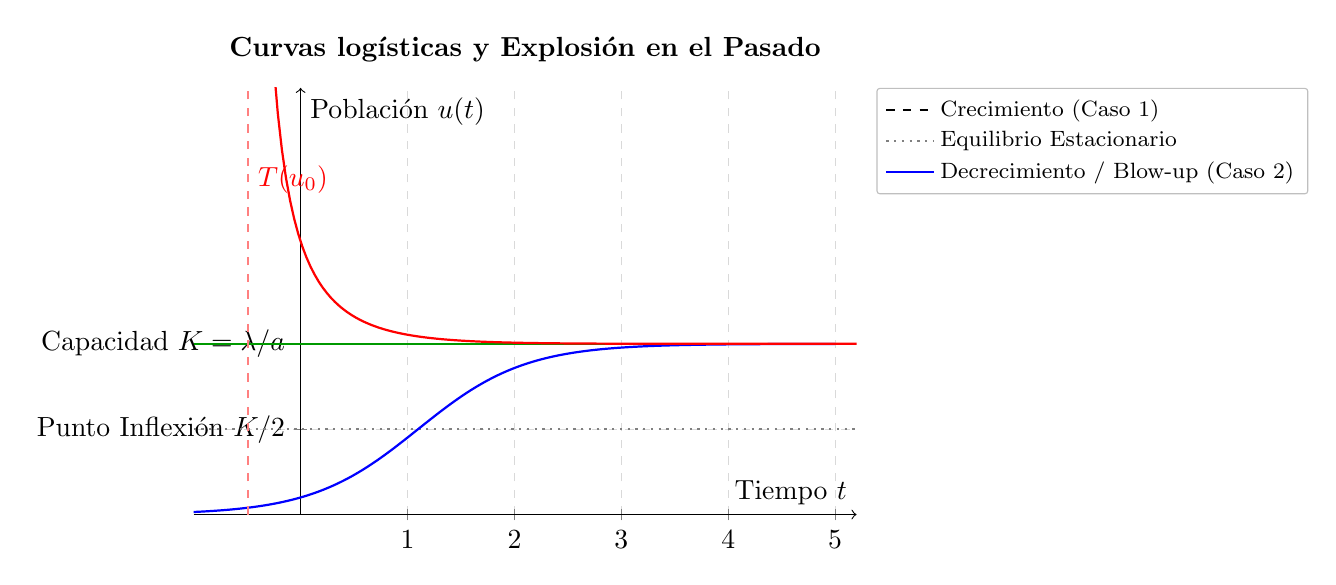
\begin{tikzpicture}
        \begin{axis}[
            width=10cm, height=7cm, % Proporciones ajustadas para dejar espacio a la leyenda
            domain=-1:5,
            samples=200,
            xmin=-1, xmax=5.2,
            ymin=0, ymax=2.5,
            xlabel={Tiempo $t$},
            ylabel={Población $u(t)$},
            axis lines=middle,
            axis line style={->}, % Flechas en los ejes
            grid=both,
            grid style={dashed, gray!30},
            xtick={0, 1, 2, 3, 4, 5},
            ytick={1, 0.5},
            yticklabels={Capacidad $K = \lambda/a$, Punto Inflexión $K/2$},
            % ---- MEJORAS DE LA LEYENDA ----
            legend pos=outer north east, % Saca la leyenda fuera del gráfico
            legend cell align={left},    % Alinea el texto a la izquierda
            legend style={
                font=\footnotesize, 
                draw=gray!50,            % Color del borde más suave
                rounded corners=1pt      % Bordes ligeramente redondeados
            },
            title={\textbf{Curvas logísticas y Explosión en el Pasado}}
        ]
        
        % Asíntota K (Capacidad de carga)
        \addplot[dashed, thick, black] coordinates {(-1,1) (5.2,1)};
        
        % Asíntota K/2 (Punto de inflexión)
        \addplot[dotted, thick, gray] coordinates {(-1,0.5) (5.2,0.5)};

        % Caso 1: Curva Sigmoide (Empieza muy baja)
        \addplot[thick, blue] { (1*0.1) / (0.1 + (1-0.1)*exp(-2*x)) };
        \addlegendentry{Crecimiento (Caso 1)}
        
        % Caso 3: Equilibrio exacto
        \addplot[thick, green!60!black] {1};
        \addlegendentry{Equilibrio Estacionario}
        
        % Caso 2/4: Superpoblación con explosión hacia atrás
        \addplot[thick, red, domain=-0.48:5.2, samples=150] { (1*1.6) / (1.6 + (1-1.6)*exp(-2*x)) };
        \addlegendentry{Decrecimiento / Blow-up (Caso 2)}
        
        % Línea asintótica vertical de explosión
        \draw[dashed, red!50!white, thick] (axis cs:-0.49,0) -- (axis cs:-0.49,2.5);
        \node[red, anchor=north west] at (axis cs:-0.49, 2.1) {$T(u_0)$};

        \end{axis}
    \end{tikzpicture}
    \end{center}

    \begin{center}
    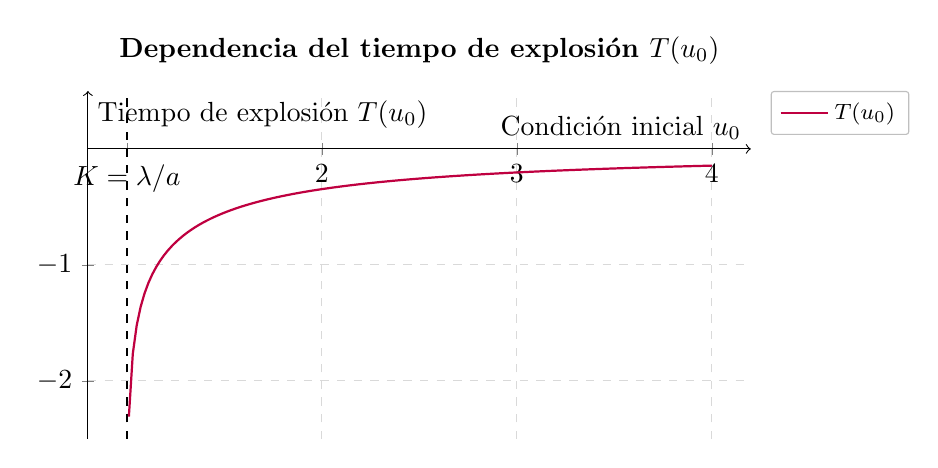
\begin{tikzpicture}
        \begin{axis}[
            width=10cm, height=6cm,
            domain=1.01:4,
            samples=150,
            xmin=0.8, xmax=4.2,
            ymin=-2.5, ymax=0.5,
            xlabel={Condición inicial $u_0$},
            ylabel={Tiempo de explosión $T(u_0)$},
            axis lines=middle,
            axis line style={->},
            grid=both,
            grid style={dashed, gray!30},
            xtick={1, 2, 3, 4},
            xticklabels={$K = \lambda/a$, $2$, $3$, $4$},
            ytick={0, -1, -2},
            % ---- MEJORAS DE LA LEYENDA ----
            legend pos=outer north east, 
            legend cell align={left},
            legend style={
                font=\footnotesize, 
                draw=gray!50, 
                rounded corners=1pt
            },
            title={\textbf{Dependencia del tiempo de explosión $T(u_0)$}}
        ]
        
        % Asíntota vertical en u0 = \lambda/a (K=1)
        \draw[dashed, thick, black] (axis cs:1,-2.5) -- (axis cs:1,0.5);
        
        % Curva del tiempo de explosión T(u_0) = 0.5 * ln(1 - 1/u_0) para lambda=2, a=2
        \addplot[thick, purple] { 0.5 * ln(1 - 1/x) };
        \addlegendentry{$T(u_0)$}

        \end{axis}
    \end{tikzpicture}
    \end{center}

    \textbf{Estudio Dinámico Cualitativo}
    
    Toda la información obtenida analíticamente se puede deducir de forma visual y elegante estudiando la ecuación como un sistema autónomo de la forma $u' = f(u)$. Definimos nuestro campo vectorial poblacional como:
    \[
        f(u) = \lambda u - a u^2 = u(\lambda - a u)
    \]
    Geométricamente, la gráfica de $f(u)$ frente a $u$ es una parábola cóncava hacia abajo. Encontraremos los puntos donde la velocidad de crecimiento es máxima calculando el punto crítico de $f(u)$:
    \[
        \frac{d}{du} f(u) = \lambda - 2 a u = 0 \implies u = \frac{\lambda}{2 a}
    \]
    Para confirmar que es un máximo, evaluamos la segunda derivada:
    \[
        \frac{d^2}{du^2} f(u) = -2 a < 0 \quad \text{(Es un máximo global de crecimiento)}
    \]
    
    Los equilibrios del sistema (puntos singulares) corresponden a las raíces del campo vectorial, $f(u) = 0$, que nos devuelve las dos soluciones constantes que ya conocíamos: $u = 0$ y $u = \lambda/a$. 
    
    El signo de $f(u)$ en los intervalos delimitados por estas raíces nos dicta la dirección del flujo de la población en la \textit{línea de fases}:
    \[
        u' = f(u) \begin{cases}
            > 0 & \text{si } 0 < u < \frac{\lambda}{a} \implies \text{Flujo hacia la derecha (población crece)} \\
            = 0 & \text{si } u = 0 \text{ o } u = \frac{\lambda}{a} \implies \text{Puntos de equilibrio} \\
            < 0 & \text{si } u > \frac{\lambda}{a} \implies \text{Flujo hacia la izquierda (población decrece)}
        \end{cases}
    \]
    Evaluando la derivada $f'(u)$ en los equilibrios determinamos su estabilidad:
    \begin{itemize}
        \item $f'(0) = \lambda > 0$. Al ser positivo, las soluciones cercanas se alejan. Es un \textbf{equilibrio inestable} (repulsor).
        \item $f'(\lambda/a) = \lambda - 2a(\lambda/a) = -\lambda < 0$. Al ser negativo, las soluciones cercanas son atraídas hacia él. Es un \textbf{equilibrio asintóticamente estable} (atractor global para cualquier $u_0 > 0$).
    \end{itemize}

}



\subsection{Ecuación de Riccati}

Para motivar la aparición de esta ecuación, consideremos nuevamente el problema diferencial no lineal general $u' = f(t,u)$. Si asumimos que la función $f$ es suficientemente regular respecto a la variable de estado $u$, podemos aproximar su comportamiento localmente utilizando su desarrollo en serie de Taylor en torno al estado nulo $u=0$:
\[
    u' = f(t,u) = f(t,0) + \frac{\partial f}{\partial u}(t,0) u + \frac{1}{2} \frac{\partial^2 f}{\partial u^2}(t,0) u^2 + \mathcal{O}(u^3)
\]
Si truncamos este desarrollo analítico reteniendo únicamente hasta el término cuadrático, estamos aproximando la dinámica general del sistema mediante una parábola en la variable $u$, cuyos coeficientes dependen exclusivamente del tiempo $t$. Esta aproximación cuadrática da lugar a una de las ecuaciones no lineales más conocidas de la física matemática.

\begin{definición}[Ecuación de Riccati]
    Llamamos \textbf{ecuación de Riccati} a toda ecuación diferencial ordinaria de primer orden y grado uno que pueda expresarse bajo la forma:
    \[
        u' = a(t) u^2 + b(t) u + c(t)
    \]
    donde $a, b, c : [\alpha, \beta] \to \mathbb{R}$ son funciones continuas en el intervalo de estudio, y $a(t) \not\equiv 0$.
\end{definición}

Analicemos rápidamente los casos límite de esta estructura:
\begin{itemize}
    \item Si $a(t) \equiv 0$, el término cuadrático desaparece y recuperamos una ecuación lineal estándar.
    \item Si $c(t) \equiv 0$, la ecuación de Riccati carece de término independiente y se reduce exactamente a una \textbf{ecuación de Bernoulli} con exponente $p = 2$ ($u' = b(t)u + a(t)u^2$), la cual ya sabemos resolver analíticamente.
\end{itemize}

Sin embargo, si $c(t) \neq 0$, nos enfrentamos a un obstáculo severo: \textbf{no existe ningún método de integración elemental general} que nos permita resolver una ecuación de Riccati arbitraria partiendo desde cero. 

La resolución analítica de esta ecuación está condicionada a un golpe de suerte o a una inspección heurística del problema: \textbf{debemos conocer de antemano una solución particular}. 

Supongamos que, por inspección o por consideraciones físicas del modelo, conocemos una solución particular $u_p(t)$ que satisface la ecuación, es decir, $u_p' = a(t)u_p^2 + b(t)u_p + c(t)$. Demostraremos que el conocimiento de esta única trayectoria $u_p(t)$ es suficiente para \textit{generar} la familia completa de soluciones del sistema.

Para ello, proponemos un cambio de variable traslacional, buscando la solución general $u(t)$ como una perturbación $v(t)$ alrededor de nuestra solución conocida:
\[
    u(t) = u_p(t) + v(t)
\]
Derivando esta expresión respecto al tiempo, obtenemos $u' = u_p' + v'$. Sustituyendo tanto $u$ como $u'$ en la ecuación de Riccati original:
\[
    u_p' + v' = a(t) \big( u_p + v \big)^2 + b(t) \big( u_p + v \big) + c(t)
\]
Desarrollando el binomio al cuadrado y aplicando la propiedad distributiva:
\[
    u_p' + v' = a(t) \big( u_p^2 + 2u_p v + v^2 \big) + b(t)u_p + b(t)v + c(t)
\]
A continuación, reordenamos algebraicamente el lado derecho de la ecuación, agrupando de manera estratégica aquellos términos que dependen exclusivamente de la solución particular $u_p$:
\[
    u_p' + v' = \underbrace{\Big[ a(t)u_p^2 + b(t)u_p + c(t) \Big]}_{\text{Ecuación para } u_p} + a(t)v^2 + \Big( 2a(t)u_p + b(t) \Big)v
\]
Por hipótesis, sabemos que $u_p(t)$ es solución de la ecuación diferencial. Por lo tanto, el término agrupado entre corchetes es exactamente igual a $u_p'$. Esto nos permite cancelar $u_p'$ en ambos miembros de la igualdad, purificando la ecuación:
\[
    v' = a(t)v^2 + \big( 2a(t)u_p(t) + b(t) \big)v
\]
Hemos logrado un resultado analítico extraordinario. El término constante $c(t)$ ha sido completamente eliminado. La nueva ecuación para la variable perturbación $v(t)$ tiene la forma:
\[
    v' = \tilde{b}(t)v + \tilde{a}(t)v^2, \quad \text{donde } \tilde{b}(t) = 2a(t)u_p(t) + b(t) \text{ y } \tilde{a}(t) = a(t)
\]
Esta última expresión es \textbf{una ecuación de Bernoulli con $p = 2$}. Por tanto, el problema insoluble se ha reducido a un problema conocido. Para hallar la solución general, bastará con aplicar el cambio de variable estándar de Bernoulli, $w = v^{1-2} = v^{-1}$, resolver la ecuación lineal resultante para $w(t)$, y finalmente deshacer la cadena de transformaciones mediante $u(t) = u_p(t) + \frac{1}{w(t)}$.
\vspace{0.5cm}

\ejemplo{
    \textbf{Ecuación de Riccati con coeficientes constantes} \\
    Consideremos la ecuación $u' = au^2 + bu + c$ con $a, b, c \in \mathbb{R}$, $a \neq 0$.
    
    Sean $\lambda, \mu$ las raíces de la ecuación $au^2 + bu + c = 0$, dadas por $u = \frac{-b \pm \sqrt{b^2-4ac}}{2a}$.
    Supongamos que son raíces reales y distintas ($\lambda \neq \mu$). Entonces podemos factorizar:
    \[
        au^2 + bu + c = a(u - \lambda)(u - \mu) \implies u' = a(u - \lambda)(u - \mu)
    \]
    Proponemos el cambio de variable de Riccati $u(t) = p(t) + v(t) = \lambda + v(t)$, ya que está claro que $p(t) = \lambda$ es una solución particular.
    Derivando y sustituyendo en la ecuación factorizada obtenemos:
    \[
        v'(t) = a(\lambda + v(t) - \lambda)(\lambda + v(t) - \mu) = a v(t) (v(t) + \lambda - \mu) = a(\lambda - \mu)v(t) + a v^2(t)
    \]
    Esto es exactamente una ecuación de Bernoulli con $\alpha = 2$. Aplicamos su cambio $w = v^{1-2} = v^{-1}$:
    \[
        -w^{-2} w' = a(\lambda - \mu)w^{-1} + a w^{-2} \implies -w' = a(\lambda - \mu)w + a \implies w' = a(\mu - \lambda)w - a
    \]
    Resolviendo esta ecuación lineal por separación, obtenemos la solución general para $w(t)$:
    \[
        w(t) = K e^{a(\mu - \lambda)t} + \frac{1}{\mu - \lambda}
    \]
    Deshaciendo los cambios de variable ($v = 1/w$ y finalmente $u = \lambda + v$), la familia de soluciones es:
    \[
        u(t) = \lambda + \frac{1}{K e^{a(\mu - \lambda)t} + \frac{1}{\mu - \lambda}}
    \]
}

\subsection{Ecuaciones en variables separables}

Son ecuaciones que se pueden escribir de la forma $u' = a(t)g(u)$.

Ejemplos: 
\begin{itemize}
    \item La ecuación de Bernoulli $u' = a(t)u + b(t)u^p$ \textbf{no} es de variables separables en general. La de Riccati tampoco.
    \item Las ecuaciones autónomas $u' = \lambda u - au^2$ o $u' = au^2 + bu + c$ sí lo son (basta tomar $a(t) = 1$ y $g(u)$ el polinomio correspondiente).
\end{itemize}

\textbf{Estudio de $u' = u^p$} con $p \neq 1$ (notemos que si $p=1$, tenemos $u' = u \implies u(t) = u_0 e^t$).

Consideremos el problema de valor inicial:
\[
    \begin{cases}
        u' = u^p \\
        u(0) = u_0 > 0
    \end{cases}
\]
Como partimos de $u(0) = u_0 > 0$, asumimos $u(t) > 0$. Separando variables:
\[
    u'(t) u^{-p}(t) = 1 \implies \left( \frac{u^{-p+1}(t)}{-p+1} \right)' = 1
\]
Integramos a ambos lados entre $0$ y $t$:
\[
    \int_0^t \left( \frac{u^{1-p}(s)}{1-p} \right)' ds = \int_0^t 1 \, ds
\]
Aplicando la regla de Barrow obtenemos:
\[
    \left[ \frac{u^{1-p}(s)}{1-p} \right]_0^t = t \implies \frac{u^{1-p}(t) - u_0^{1-p}}{1-p} = t
\]
Despejando $u(t)$:
\[
    u^{1-p}(t) = u_0^{1-p} + (1-p)t \implies u(t) = \left[ u_0^{1-p} + (1-p)t \right]^{\frac{1}{1-p}}
\]
Esta es la única solución.
\begin{itemize}
    \item \textbf{Caso 1: $p > 1$ (Explosión en tiempo finito)} \\
    Si $p > 1$, entonces el factor $(1-p)$ es negativo. Como partimos de $u_0 > 0$ y $u' = u^p > 0$, la función es estrictamente creciente. Además, su segunda derivada $u'' = p u^{p-1} u' > 0$, lo que indica un crecimiento estrictamente convexo (acelerado).
    
    Dado que el exponente global de la solución $\frac{1}{1-p}$ es negativo, equivale a tener el corchete en un denominador. La solución dejará de existir (explotará a infinito) en el instante de tiempo en el que dicho corchete se anule:
    $$ u_0^{1-p} + (1-p)t = 0 \implies t = \frac{-u_0^{1-p}}{1-p} = \frac{1}{(p-1)u_0^{p-1}} $$
    Este valor temporal es estrictamente positivo. Por lo tanto, definimos el \textbf{tiempo de explosión} ($T_{max}$) como:
    $$ T_{max}(u_0) = \frac{1}{p-1} \frac{1}{u_0^{p-1}} $$
    En este caso, $\lim_{t \to T_{max}^-} u(t) = +\infty$. La solución no es global, solo está definida en el intervalo finito $[0, T_{max})$.
    Además, observamos los límites:
    \[
        \lim_{u_0 \to 0} T_{max}(u_0) = +\infty, \quad \lim_{u_0 \to +\infty} T_{max}(u_0) = 0
    \]

    \begin{center}
    \begin{tikzpicture}
        \begin{axis}[
            width=7cm, height=5cm,
            xmin=-0.5, xmax=4,
            ymin=0, ymax=5,
            axis lines=middle,
            xlabel={$t$},
            ylabel={$u(t)$},
            xtick={3},
            xticklabels={$T_{max}(u_0)$},
            ytick={1},
            yticklabels={$u_0$},
            every axis x label/.style={at={(ticklabel* cs:1)},anchor=west},
            every axis y label/.style={at={(ticklabel* cs:1)},anchor=south},
        ]
        % Asíntota vertical
        \draw[dashed, thick, red!70!black] (axis cs:3,0) -- (axis cs:3,5);
        % Curva de explosión (Blow-up)
        \addplot[thick, blue, domain=0:2.85, samples=100] {1/(1 - x/3)};
        \end{axis}
    \end{tikzpicture}
    \end{center}

    \item \textbf{Caso 2: $0 < p < 1$ (Existencia global y pérdida de unicidad)} \\
    Si $0 < p < 1$, entonces el factor $(1-p)$ es positivo. En este escenario, el término $(1-p)t$ suma positivamente a $u_0^{1-p}$. El corchete jamás se anula para $t \ge 0$, por lo que la solución no explota y está \textbf{definida globalmente} para todo $t \in [0, +\infty)$ y es monótona creciente.
    
    ¿Qué ocurre si tomamos el límite para una condición inicial nula, es decir, $u_0 \to 0$?
    $$ \lim_{u_0 \to 0} u(t; u_0) = \Big[ (1-p)t \Big]^{\frac{1}{1-p}} =: \varphi(t) $$
    Es inmediato comprobar que esta función $\varphi(t)$ resuelve la ecuación $u' = u^p$ con $\varphi(0) = 0$. 
    Sin embargo, la solución trivial $u \equiv 0$ también resuelve el mismo problema $u' = u^p$ con $u(0) = 0$. 
    Por lo tanto, \textbf{ya no hay unicidad}, y tenemos por lo menos 2 soluciones válidas.

    \begin{center}
    \begin{tikzpicture}
        \begin{axis}[
            width=7cm, height=5cm,
            xmin=-0.5, xmax=4,
            ymin=-0.5, ymax=4,
            axis lines=middle,
            xlabel={$t$},
            ylabel={$u(t)$},
            xtick=\empty,
            ytick=\empty,
            every axis x label/.style={at={(ticklabel* cs:1)},anchor=west},
            every axis y label/.style={at={(ticklabel* cs:1)},anchor=south},
        ]
        % Solución nula
        \addplot[thick, red!80!black, domain=0:4] {0} node[pos=0.8, below] {$u \equiv 0$};
        % Solución phi(t)
        \addplot[thick, blue, domain=0:2, samples=100] {x^1.5} node[pos=0.8, left] {$\varphi(t)$};
        \end{axis}
    \end{tikzpicture}
    \end{center}
\end{itemize}


\ejemplo{
    \textbf{Patología 1: Pérdida de unicidad (Caso $0 < p < 1$)}\\
    Consideremos el siguiente problema de valor inicial:
    \[
        \begin{cases}
            u' = u^p, \quad 0 < p < 1 \\
            u(0) = u_0 > 0
        \end{cases}
    \]
    Notemos que si $p = 1/2$, obtenemos la ecuación $u' = \sqrt{u}$. La función $g(u) = \sqrt{u}$ es continua en todo su dominio, pero su derivada diverge en el origen, por lo que no es localmente Lipschitz (no es diferenciable en $u=0$).
    
    Para resolverla analíticamente, separamos las variables e integramos a ambos lados respecto al tiempo:
    \[
        u'(t) u^{-p}(t) = 1 \implies \frac{d}{dt} \left( \frac{u^{1-p}(t)}{1-p} \right) = 1 
    \]
    Integrando directamente, obtenemos:
    \[
        \frac{u^{1-p}(t)}{1-p} = t + C 
    \]
    Imponiendo la condición inicial $u(0) = u_0$, deducimos el valor de la constante de integración:
    \[
        \frac{u_0^{1-p}}{1-p} = 0 + C \implies C = \frac{u_0^{1-p}}{1-p} 
    \]
    Sustituyendo $C$ en la expresión y multiplicando todo por $(1-p)$:
    \[
        u^{1-p}(t) = (1-p)t + u_0^{1-p} \implies u(t) = \left( (1-p)t + u_0^{1-p} \right)^{\frac{1}{1-p}}
    \]
    Dado que $1-p > 0$, esta función crece indefinidamente: $\lim_{t \to +\infty} u(t) = +\infty$.
    
    El fenómeno patológico ocurre si evaluamos el caso particular donde partimos del reposo, $u_0 = 0$. El problema de Cauchy:
    \[
        \begin{cases}
            \varphi' = \varphi^p \\
            \varphi(0) = 0
        \end{cases} 
    \]
    posee, a simple vista, la solución trivial estacionaria $\varphi(t) \equiv 0$. Sin embargo, la fórmula que acabamos de deducir nos proporciona otra solución válida válida para $t \geq 0$:
    \[
        \varphi(t) = \big( (1-p)t \big)^{\frac{1}{1-p}}
    \]
    Ambas funciones satisfacen la ecuación y la condición inicial. De hecho, podemos empalmar estas soluciones para crear una \textbf{familia uniparamétrica infinita de soluciones} parametrizada por un tiempo de despegue $\tau \geq 0$:
    \[
        \varphi_\tau (t) := \begin{cases}
            0 & \text{si } 0 \leq t < \tau \\
            \big( (1-p)(t-\tau) \big)^{\frac{1}{1-p}} & \text{si } t \geq \tau
        \end{cases}
    \]
    Concluimos que en los sistemas no lineales, la simple continuidad de $f(t,u)$ no es suficiente para garantizar la unicidad de la solución.
}

\ejemplo{
    \textbf{Patología 2: Explosión en tiempo finito / Blow-up (Caso $p > 1$)}\\
    Estudiemos ahora qué ocurre cuando la no linealidad es muy fuerte ($p > 1$), añadiendo además un decaimiento exponencial en el tiempo. Sea el problema:
    \[
        \begin{cases}
            u' = e^{-t} u^p, \quad p > 1 \\
            u(0) = u_0 > 0
        \end{cases}
    \]
    Esta ecuación es separable con $a(t) = e^{-t}$ y $g(u) = u^p$. Para instantes iniciales $t$ próximos a $0$, la solución $u(t) \sim u_0 > 0$, manteniéndose positiva. Separando variables:
    \[
        u^{-p}(t) u'(t) = e^{-t} \implies \frac{d}{dt} \left( \frac{u^{1-p}(t)}{1-p} \right) = e^{-t}
    \]
    Integrando:
    \[
        \frac{u^{1-p}(t)}{1-p} = -e^{-t} + C 
    \]
    Imponiendo la condición inicial $u(0) = u_0$:
    \[
        \frac{u_0^{1-p}}{1-p} = -1 + C \implies C = \frac{u_0^{1-p}}{1-p} + 1
    \]
    Sustituimos $C$ y multiplicamos toda la ecuación por el factor $(1-p)$. Es crucial notar aquí que, como $p > 1$, el término $(1-p)$ es una cantidad \textbf{estrictamente negativa}.
    \begin{align*}
        u^{1-p}(t) &= (1-p)(-e^{-t} + 1) + u_0^{1-p} \\
        \frac{1}{u^{p-1}(t)} &= u_0^{1-p} + (1-p)(1 - e^{-t})
    \end{align*}
    Elevando todo a la potencia inversa, obtenemos la solución explícita:
    \[
        u(t;0,u_0) = \Big( u_0^{1-p} + (1-p)(1 - e^{-t}) \Big)^{\frac{1}{1-p}} = \frac{1}{\Big( u_0^{1-p} + (1-p)(1 - e^{-t}) \Big)^{\frac{1}{p-1}}}
    \]
    Veamos cómo se comporta esta solución a medida que avanza el tiempo. La base del exponente en el denominador es $f(t) = u_0^{1-p} + (1-p)(1 - e^{-t})$. Cuando $t \to +\infty$, el término exponencial desaparece, por lo que:
    \[
        f(t) \xrightarrow{t \to +\infty} u_0^{1-p} + (1-p)
    \]
    Para que la solución exista globalmente para todo tiempo $t \in [0, +\infty)$, necesitamos garantizar que el denominador no se anule ni se vuelva negativo, lo que equivale a exigir que el límite asintótico sea estrictamente positivo:
    \[
        u_0^{1-p} + (1-p) > 0 \implies u_0^{1-p} > p-1 \implies u_0 < \left(\frac{1}{p-1}\right)^{\frac{1}{p-1}} \equiv u_0^*
    \]
    Se abren entonces dos regímenes dinámicos totalmente distintos dependiendo de la magnitud de nuestra condición inicial $u_0$:
    
    \begin{itemize}
        \item \textbf{Régimen de existencia global ($u_0 < u_0^*$):} Si partimos de una población inferior al umbral crítico $u_0^*$, el denominador se mantiene siempre positivo. La solución está definida para todo tiempo $t \geq 0$ y su límite a largo plazo es una constante finita que depende del estado inicial:
        \[
            \lim_{t \to +\infty} u(t;0,u_0) = \omega(u_0) = \Big( u_0^{1-p} + (1-p) \Big)^{\frac{1}{1-p}}
        \]
        Notemos que si nos acercamos peligrosamente al umbral por la izquierda ($u_0 \uparrow u_0^*$), la base tiende a $0$ y el límite asintótico diverge: $\lim_{u_0 \uparrow u_0^*} \omega(u_0) = +\infty$.

        \item \textbf{Régimen de explosión o Blow-up ($u_0 > u_0^*$):} Si superamos el umbral crítico, existirá irremediablemente un instante $T$ en el que el denominador de nuestra solución se anulará:
        \[
            u_0^{1-p} + (1-p)(1 - e^{-T}) = 0
        \]
        Cuando el tiempo se acerca a este instante ($t \uparrow T$), la función diverge a infinito:
        \[
            \lim_{t \uparrow T} u(t;0,u_0) = +\infty
        \]
        Este fenómeno se denomina \textbf{explosión en tiempo finito}. Despejando $T$, hallamos el tiempo exacto de vida de la solución:
        \[
            T(u_0) = -\ln\left( 1 + \frac{u_0^{1-p}}{1-p} \right) > 0
        \]
    \end{itemize}
}

\begin{observación}[Condición general de explosión]
    Consideremos la ecuación general $u' = a(t) u^p$ con $p > 1$ y $u_0 > 0$. Asumiendo $a: [0, +\infty) \to [0, +\infty)$ continua, la aparición del blow-up está gobernada por la integral impropia del factor temporal:
    \[
        \int_0^{+\infty} a(s) ds = I
    \]
    \begin{itemize}
        \item Si la integral es convergente ($I < +\infty$), como ocurrió en el ejemplo previo con $a(t) = e^{-t}$, el sistema tiene capacidad de "frenar" la explosión si la condición inicial es suficientemente pequeña.
        \item Si la integral es divergente ($I = +\infty$), como ocurre si $a(t) = 1$ o $a(t) = t$, la ecuación forzará invariablemente a la solución a explotar en tiempo finito, sin importar cuán pequeño sea el valor inicial $u_0 > 0$.
    \end{itemize}
\end{observación}

\subsection{Teoría fundamental de las variables separables}

Comprendidas las patologías que pueden surgir si la función no es suficientemente regular, podemos formalizar el teorema central que garantiza la resolución analítica y segura de estas ecuaciones.

\begin{teorema} [Teorema Fundamental de existencia y unicidad para ecuaciones de variables separables]
    Sean $t_0, u_0 \in \mathbb{R}$. Consideremos dos funciones continuas en entornos de las condiciones iniciales: una función temporal $a : [t_0 - \nu, t_0 + \nu] \to \mathbb{R}$ (con $\nu > 0$) y una función espacial $g : [u_0 - R, u_0 + R] \to \mathbb{R}$ (con $R > 0$). 
    
    Si imponemos la condición de regularidad estricta $g(u_0) \neq 0$, entonces el Problema de Valor Inicial:
    \[
        P = \begin{cases}
            u' = a(t) g(u) \\
            u(t_0) = u_0
        \end{cases}
    \]
    tiene una \textbf{única solución local}. Es decir, existe un radio $\varepsilon > 0$ tal que existe una única función $u \in C^1((t_0 - \varepsilon, t_0 + \varepsilon), \mathbb{R})$ que resuelve el P.V.I. para todo $t \in (t_0 - \varepsilon, t_0 + \varepsilon)$.
\end{teorema}

\begin{observación}
    Es absolutamente crucial la hipótesis $g(u_0) \neq 0$. Si por el contrario $g(u_0) = 0$, la función constante $u(t) \equiv u_0$ es trivialmente una solución de equilibrio. Sin embargo, no podemos garantizar que sea la única. El clásico contraejemplo es $u' = \sqrt{|u|}$ con $u(0) = 0$ (donde $a(t)=1$, $g(u) = \sqrt{|u|}$ y $g(0)=0$), el cual, como vimos en la Patología 1, posee infinitas soluciones bifurcadas.
\end{observación}

\begin{proof}
    Como suponemos $g(u_0) \neq 0$, por continuidad de $g$ e imponiendo continuidad en nuestra solución incógnita $u(t)$, sabemos que para $t \sim t_0$ se cumple que $u(t) \sim u(t_0) = u_0$. En consecuencia, $g(u(t))$ mantendrá su signo y no se anulará en un entorno local: $g(u(t)) \sim g(u_0) \neq 0$. 
    
    Esto nos otorga legitimidad algebraica para dividir la ecuación original $u'(t) = a(t) g(u(t))$ por $g(u(t))$:
    \[
        \frac{u'(t)}{g(u(t))} = a(t)
    \]
    Aplicando la regla de la cadena y el Teorema Fundamental del Cálculo, podemos identificar el lado izquierdo como la derivada temporal de una integral acumulada. Integrando ambos miembros desde el instante $t_0$ hasta $t$:
    \[
        \frac{d}{dt} \left( \int_{u_0}^{u(t)} \frac{1}{g(s)} ds \right) = a(t)  \iff \int_{u_0}^{u(t)} \frac{1}{g(s)} ds = \int_{t_0}^t a(s) ds
    \]
    Por tanto, $u(t)$ es solución del problema diferencial $P$ si y solo si es solución de la ecuación integral implícita anterior. Para demostrar que esta ecuación define una única función local $u(t)$, definimos la función bivariada:
    \[
        H(u,t) \equiv \int_{u_0}^{u} \frac{1}{g(s)} ds - \int_{t_0}^t a(s) ds, \quad \text{definida para } u \sim u_0, \ t \sim t_0
    \]
    La ecuación integral equivale a hallar las curvas de nivel $H(u,t) = 0$. Evaluamos la regularidad de $H$. Derivando respecto a sus dos variables mediante el Teorema Fundamental del Cálculo:
    \[
        \frac{\partial H}{\partial u} (u,t) = \frac{1}{g(u)} \quad \text{(es continua)} \qquad \frac{\partial H}{\partial t} (u,t) = -a(t) \quad \text{(es continua)}
    \]
    Luego $H$ es una función de clase $C^1$ en un entorno de $(u_0, t_0)$. Además, evaluando en el punto inicial comprobamos que la ecuación se satisface: $H(u_0, t_0) = 0 - 0 = 0$. 
    
    Por último, verificamos la condición transversal del Teorema de la Función Implícita:
    \[
        \frac{\partial H}{\partial u} (u_0, t_0) = \frac{1}{g(u_0)} \neq 0
    \]
    Como la derivada parcial respecto a la variable incógnita no se anula, el \textbf{Teorema de la Función Implícita} nos garantiza concluyentemente la existencia de un $\varepsilon > 0$ y de una única función explícita $u : [t_0 - \varepsilon, t_0 + \varepsilon] \to \mathbb{R}$ de clase $C^1$, tal que $u(t_0) = u_0$ y $H(u(t), t) = 0$ para todo $t$ en el entorno. Por ende, $u(t)$ es la única solución local del problema diferencial original.
\end{proof}

\ejemplo{
    Aplicaremos la técnica recién demostrada para resolver el siguiente y vistoso problema de variables separables:
    \[
        \begin{cases}
            u' = \sqrt{u (\pi - u)} \\
            u(0) = u_0 \in (0, \pi)
        \end{cases}   
    \]
    *(Nota: Modelos similares surgen en dinámica de poblaciones restringidas, variaciones como $u' = t \sqrt{u (\pi - u)}$ o formas genéricas $u' = \sqrt{(u - \omega_1)(\omega_2 - u)}$ se resuelven mediante el mismo armazón analítico).*

    Vamos a nuestro problema original. Identificamos la función no lineal $g(u) = \sqrt{u(\pi - u)}$. Esta función es continua en el dominio cerrado $[0, \pi]$. Sin embargo, observemos que sus derivadas divergen en las fronteras: $g'(0) = +\infty$ y $g'(\pi) = -\infty$, lo que advierte de una pérdida de regularidad extrema si el sistema tocara esos bordes. 
    
    Afortunadamente, partimos de un estado inicial interior $u_0 \in (0, \pi)$, lo que garantiza que $g(u_0) \neq 0$. Por el Teorema Fundamental recién demostrado, sabemos con total certeza que \textbf{tiene una única solución local}.
    
    Para $t \sim 0$, $u(t) \sim u_0$, la función se mantiene lejos de las fronteras problemáticas y podemos separar variables dividiendo la ecuación:
    \[  
        \frac{u'(t)}{\sqrt{u(t)(\pi - u(t))}} = 1 \implies \frac{d}{dt} \left( \int_{u_0}^{u(t)} \frac{1}{\sqrt{s(\pi - s)}} ds \right) = 1
    \]
    Integrando a ambos lados respecto al tiempo, obtenemos la forma implícita:
    \[
        \int_{u_0}^{u(t)} \frac{1}{\sqrt{s(\pi - s)}} ds = t
    \]
    Para resolver la integral irracional del lado izquierdo, recurrimos al clásico método de completar cuadrados en el radicando:
    \begin{align*}
        s(\pi - s) &= \pi s - s^2 \\
        &= - \left( s^2 - 2 \left(\frac{\pi}{2}\right) s \right) \\
        &= - \left( s^2 - 2 \left(\frac{\pi}{2}\right) s + \left(\frac{\pi}{2}\right)^2 - \left(\frac{\pi}{2}\right)^2 \right) \\
        &= \left(\frac{\pi}{2} \right)^2 - \left(s - \frac{\pi}{2} \right)^2 
    \end{align*}
    Para facilitar la integración, factorizamos la constante $(\pi/2)^2$ del bloque:
    \[
        s(\pi - s) = \left(\frac{\pi}{2} \right)^2 \left[ 1 - \left(\frac{s - \frac{\pi}{2}}{\frac{\pi}{2}} \right)^2 \right] 
    \]
    Sustituyendo esto dentro de la raíz en nuestra integral, el cuadrado del exterior sale de la raíz como $\pi/2$:
    \[
        \int_{u_0}^{u(t)} \frac{1}{\frac{\pi}{2} \sqrt{1 - \left(\frac{s - \frac{\pi}{2}}{\frac{\pi}{2}} \right)^2}} ds = t
    \]
    Realizamos el sutil cambio de variable trigonométrico interno $w = \frac{s - \pi/2}{\pi/2}$, donde reconocemos inmediatamente que $dw = \frac{ds}{\pi/2}$. La integral se reduce, por arte de magia algebraica, a la derivada canónica del arcoseno:
    \[
        \int_{w(u_0)}^{w(u(t))} \frac{1}{\sqrt{1 - w^2}} dw = t \implies \Big[ \arcsin(w) \Big]_{w(u_0)}^{w(u(t))} = t
    \]
    Evaluando en los límites, la relación implícita se concreta en:
    \[
        \arcsin \left( \frac{u(t) - \frac{\pi}{2}}{\frac{\pi}{2}} \right) - \arcsin \left( \frac{u_0 - \frac{\pi}{2}}{\frac{\pi}{2}} \right) = t
    \]
    Para hallar la solución explícita, aislamos el término de $u(t)$, pasando la constante inicial sumando al tiempo, y aplicamos la función seno a ambos miembros de la ecuación:
    \[
        \frac{u(t) - \frac{\pi}{2}}{\frac{\pi}{2}} = \sin\left( t + \arcsin \left( \frac{u_0 - \frac{\pi}{2}}{\frac{\pi}{2}} \right) \right)
    \]
    Despejando finalmente la incógnita temporal $u(t)$, coronamos el análisis con la preciosa solución explícita oscilatoria:
    \[
        \boxed{u(t) = \frac{\pi}{2} \sin\left( t + \arcsin \left( \frac{2u_0 - \pi}{\pi} \right) \right) + \frac{\pi}{2}}
    \]
}